\section{Method}
\label{sec:method}

\subsection{Setting}
\label{sec:setting}

We work in \simname, an internal high-fidelity closed-loop driving simulator whose \emph{official scene score} $y\in[0,1]$ aggregates safety, compliance, and progress into a single scalar per rollout.
The official score is the \emph{sole} selection supervision: submetric aggregates are deliberately barred from the selector's objective to prevent the selector from gaming individual submetrics---consequence submetrics enter only as auxiliary heads (\cref{sec:head}).
Each scene contributes three \emph{decision groups} at staggered decision times (timing tags A/B/C).
For each group, the frozen generator \vlaname{} (10B) samples $K{=}8$ candidate trajectories from one prompt prefill; every candidate is then executed in closed loop and receives its own official score, giving $3\times8=24$ scoring rollouts per scene and \nScoresTotal{} candidate-level scores on the \nScenes-scene primary cohort (\nGroups{} groups).

Given a group $g$ with candidates $c_1,\dots,c_K$ and scores $y(c_k)$, a selector $\pi$ picks $\hat c=\pi(g)$.
Our two co-primary endpoints are
\emph{selected regret}, $\regret(g) = \max_k y(c_k) - y(\hat c)$ (lower is better; the oracle-selector gap actually paid at deployment), and
\emph{tie-aware top-1 agreement}, $\mathbf{1}[\,y(\hat c) \ge \max_k y(c_k) - \epsilon\,]$ with $\epsilon=\TieEps$ (higher is better).
Both aggregate group $\rightarrow$ scene mean (3 groups) $\rightarrow$ seed mean $\rightarrow$ paired scene bootstrap (\cref{sec:protocol}).

\subsection{Same-prefill capture}
\label{sec:capture}

A representation-reuse claim is confounded if the representation could come from a \emph{different} forward pass than the candidates (different context window, different preprocessing, silently re-run prefill).
We eliminate this by construction: a capture hook inside the production \texttt{predict()} path records the final transformer layer's hidden states (post final normalization) of the prompt prefill, $H\in\mathbb{R}^{3086\times4096}$ (the prompt length is invariant across groups), \emph{during the same call} that samples the $K$ candidates, with an exactly-one-prefill assertion so a second prefill in the call would fail the capture rather than silently substitute context.
The pooled scene vector used at deployment is the last row, $h = H_{3086}\in\mathbb{R}^{4096}$; capture-time SHA-256 hashes of both tensors establish bit-exact provenance ($h \equiv H[-1]$ verified for \nGroups/\nGroups{} groups), and every downstream artifact (training tables, locked predictions, analysis JSONs) carries these hashes forward.
\Cref{fig:capture} summarizes the chain.
Candidates, representation, and scores are therefore certifiably co-produced---the ablations in \cref{sec:res-signal} then test whether the representation's \emph{content} matters.

\begin{figure}[t]
  \centering
  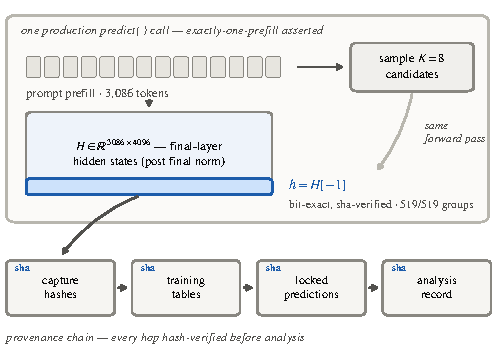
\includegraphics[width=\linewidth]{figs/fig_capture.pdf}
  \caption{\textbf{Same-prefill capture and provenance.} One production \texttt{predict()} call per decision group: the 3{,}086-token prompt prefill produces both the $K{=}8$ sampled candidates and the captured final-layer hidden states $H$; the deployed scene vector is bit-exactly $h=H[-1]$ (SHA-256 verified at capture, \nGroups/\nGroups{} groups). Every downstream artifact---training tables, locked predictions, the analysis record---carries the hashes forward.}
  \label{fig:capture}
\end{figure}

\subsection{Selector head}
\label{sec:head}

\begin{figure*}[t]
  \centering
  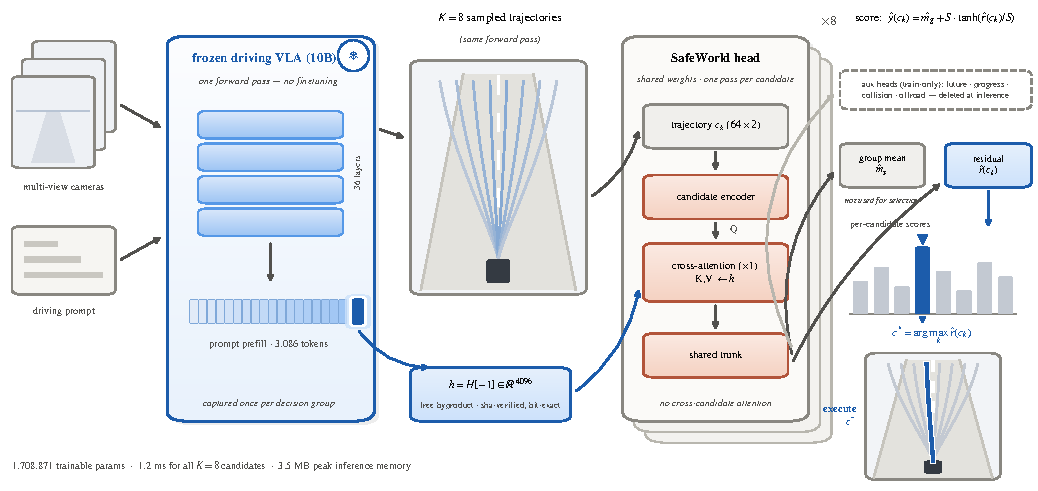
\includegraphics[width=\textwidth]{figs/fig_arch.pdf}
  \caption{\textbf{Architecture.} One frozen forward pass of \vlaname{} yields both the $K{=}8$ candidate trajectories and the prefill hidden states $H$; the only representation consumed downstream is the last row $h=H[-1]$, a free byproduct of generation. The \headname{} head (\EffParams{} parameters---the only trained component) runs once per candidate with shared weights: a candidate encoder queries $h$ through a single cross-attention block into a shared trunk. The score decomposes into a group mean $\hat m_g$ (excluded from selection) and a bounded residual $\hat r$ that alone drives the selector (\cref{eq:decomp}); the selected trajectory is executed. Auxiliary consequence heads are training-only---deleted at inference, the deployed score is bit-identical. Per-candidate scores and trajectories in the panel are illustrative.}
  \label{fig:arch}
\end{figure*}

The \headname{} head (\cref{fig:arch}; \EffParams{} trainable parameters; the frozen VLA receives no gradients) scores each candidate independently---no cross-candidate attention, so scores are $K$-invariant and permutation-equivariant by construction (verified: off-diagonal cross-candidate gradients are exactly zero; scores are bit-identical alone or batched).
A candidate encoder embeds the trajectory; a single cross-attention block queries the scene representation (the last token $h$, or in ablation arms the full sequence $H$); shared trunk features feed the output heads.

\paragraph{Decomposed score.}
Naively regressing $y$ conflates two signals of very different scale: the group's overall difficulty and the candidate's \emph{relative} quality within the group---and only the latter matters for selection.
Earlier design-phase studies in this program showed the conflation concretely: an unconstrained residual develops gradient conflict between ranking and centered-regression losses, and group-level offsets dominate the representation.
We therefore decompose
\begin{equation}
  \hat y(c) \;=\; \hat m_g \;+\; S\,\tanh\!\big(\hat r(c)/S\big),
  \qquad S=0.67,
  \label{eq:decomp}
\end{equation}
where $\hat m_g$ is a group-mean head, $\hat r(c)$ is a per-candidate residual (zero-initialized), and the bound $S$ (frozen from development-cohort residual statistics) keeps the residual inside the empirically observed spread.
The deployed selector is $\hat c=\arg\max_c \hat r(c)$: the group-mean head is excluded from selection by construction, so scene difficulty cannot leak into the choice.

\paragraph{Amortized consequence knowledge.}
Auxiliary heads predict per-candidate consequences: future ego trajectory ($64\times2$), progress, collision, and offroad.
They are \emph{training-only}: at inference the deployed score is bit-identical with the auxiliary heads deleted (a deletion test in the conformance suite).
This is the operational sense in which the selector holds \emph{amortized} world knowledge---consequences shape the representation during training but are never simulated, predicted, or consumed at decision time, in contrast to explicit-imagination designs~\cite{li2025wote}.

\subsection{Objectives}
\label{sec:objectives}

All representation arms share one architecture and parameter count (state dicts are interchangeable); arms differ only in scene-input visibility and objective.
The \emph{checkpoint objective} (used by all arms for model selection during training) is
$L = 1.0\,L_{\text{rank}} + 0.5\,L_{\text{centered}} + 0.1\,L_{\text{group-mean}} + 0.25\,L_{\text{future}} + 0.1\,L_{\text{progress}} + 0.1\,L_{\text{collision}} + 0.1\,L_{\text{offroad}}$,
with a weighted pairwise softplus ranking loss and scale-matched SmoothL1 regressions.

\paragraph{Selector loss.}
Ranking all $K$ candidates well is not the deployed task; putting the \emph{best} candidate on top is.
The selector objective replaces $L_{\text{rank}}$ (coefficient moved to 0) with a regret-weighted best-vs-rest logistic loss.
With tied-best set $B_g=\{i: y_{\max}-y_i\le\epsilon\}$ and per-candidate selector scores $s$,
\begin{equation}
  L_{\text{sel}} \;=\; \frac{\sum_{g}\sum_{i\in B_g}\sum_{j\notin B_g} \frac{w_j}{|B_g|}\,
  \mathrm{softplus}\!\big({-}(s_i-s_j)/\tau\big)}{\sum_g \sum_{j\notin B_g} w_j},
  \qquad w_j = y_{\max}-y_j,
  \label{eq:selloss}
\end{equation}
so each mistake is weighted by exactly the regret it would cost.
Both scalars are resolved \emph{mechanically} from frozen target metadata, not tuned: $\tau=\SelTau$ is the (0.001-ceiled) median positive oracle-best-to-candidate score gap, and the coefficient $\SelCoef$ equalizes the RMS per-candidate gradient $\partial L/\partial s$ against the replaced ranking term at equal scores.

\paragraph{Why not expected regret?}
The natural alternative---minimizing the expected regret of a softmax policy, $L_A=\mathbb{E}_{q}[r]$ with $q=\mathrm{softmax}(s/\tau)$---was rejected on a closed, preregistered criterion: its gradient $\partial L_A/\partial s_j = \tfrac{1}{\tau}q_j(r_j-\mathbb{E}_q[r])$ \emph{vanishes} as $q$ collapses onto a single candidate, i.e.\ exactly when the selector is \emph{confidently wrong}---the one failure mode the objective exists to repair.
The best-vs-rest logistic instead \emph{saturates at its maximum} there.
In the operating regime our development runs actually produce (within-group score spreads routinely $2.6$--$10\times$ $\tau$), the softmax gradient retains as little as $3.9\%$ of its small-spread magnitude; reproduced synthetically in the preregistration conformance suite, the softmax gradient norm collapses to \SelGradVanish{} while the frozen selector loss holds \SelGradSat.
This geometry, not any real-model outcome comparison, fixed the objective before the confirmatory studies ran (derivation and the full 12-criterion resolution in the supplement).

\subsection{Protocol}
\label{sec:protocol}

Every confirmatory study follows one frozen protocol.
\textbf{Training/evaluation:} 5-fold cross-validation split by scene $\times$ 3 seeds; checkpoint selection uses \emph{inner-validation only} (\textsc{constrained-selector-first} rule; the test fold is never consulted).
\textbf{Locking:} all per-candidate predictions for every arm and every ablation condition are hash-locked \emph{before} any endpoint is computed; the analyzer verifies every hash (and its own code hash against the registered one) and runs exactly once.
\textbf{Statistics:} paired scene percentile bootstrap, $10{,}000$ resamples, frozen seed; undefined scenes are dropped and counted, never zero-filled; we report 95\% CIs throughout and treat an effect as supported only when its CI excludes zero.
\textbf{Preregistration:} arms, endpoints, gates, margins, ablation mappings, and analysis code are frozen and hash-registered before outcomes exist; deviations would be visible as hash breaks.
